% !TeX spellcheck = en_US
% !TeX root = main.tex

\section{Aesthetics}
\subsection{Style Guide}
% Summarise the general aesthetic you've chosen and your design intentions
% How does your visual aesthetic engage your specific target audience?
% Visualise (with contextual examples):
% - Which color scheme did you use? Include HEX codes
% - Describe your text treatments. Include font names, sizes and weights
% - Describe any image or icon treatments
% - Describe any button/link treatments (e.g. hovering on a link)
% Rationalise the design choices you've made, relating to the design principles from the lectures

\subsubsection{Colour Scheme}\label{sec:color}
When picking a colour scheme it is important to take into consideration the effects the colours will have on people, also known as the colour psychology. Brown represents strength and reliability, meanwhile orange represents enthusiasm and attention. All of these traits are traits that are either associated with \gls{git} or can be used to maintain people's interest. Therefore the primary colour of the website is part the way between brown and orange to attempt to get a blend of these traits. Finally the primary colour also represents a gold style colour to better represent the value of using \gls{git}, since gold is associated with money and wealth.~\cite{colors}\\\\
A secondary colour was chosen to represent calming in order to make sure that the user never got too anxious over the content being presented to them. However after user testing and evaluation it was obvious that the users did not reach a point that the colour was required.~\cite{colors}\\\\
The background colour chosen is based on a darker shade of the primary colour, this is to help make the background a lesser focus of the content and make the content the frontmost focus of the user. This colour is meant to complement both the content background and the primary colour used in the content. The colour difference between the background and primary should be a noticeable difference but not something immediately obvious and distracting to an average consumer.\\\\
The main goal is the use of colour between; the immediate content (headings and title blocks), the content (the main information and reason the user is visiting the page), and the background. Therefore content and colours used for the content is the blending piece between the background colour and primary colour. Another consideration for the content colours is the use of dark text or light text and the effects on readers. In order to not strain the users's eyes when reading and to enforce proper reading and not skimming, a light background with dark text approach was taken~\cite{text}. Therefore a white background with black text scheme was chosen for the content.\\\\
An area of content my have particle highlighted areas which are of interest to readers if they are quickly scrolling or skimming through the content. These areas are of interest but should not distract from normal reading consumption. A slight grey tinge background with a medium sized margin around the highlighted content will help to ensure the content is well recognisable to quick reads but not distracting to normal readers. This grey combined with the primary colour on titles allows users to see the code block and then immediately identify the content.\\\\
The final \gls{html} \gls{hex} codes are as follows:
\begin{description}
	\item[Primary:] \#A18613
	\item[Secondary:] \#1975FF
	\item[Background:] \#6D532D
	\item[Content Text:] black
	\item[Content Background:] white
\end{description}

\begin{note}{Content Colouring Code}
	The use of ``black'' and ``white'' as the content colours allows for \gls{os} overrides to adjust the text, so if the user has any preferences that modify the default values of websites than these preferences will be applied to the content. The drawback of using this type of referencing means that there are varied results across browsers and systems.
\end{note}

\subsubsection{Font Families}
The font chosen is an \gls{opensource} font by Adobe, Source Sans Pro. It is a sans serif based typeface and the first Adobe \gls{opensource} font family. The font is intended to be used on user interfaces. This font is easy to read and understand and allows for users to both sit down and read and quickly skim through text without strain.~\cite{font}\\\\
A typewriter based font is used as a secondary font for identifying blocks of code within paragraphs. This font was used because of it recognition to code based fonts and terminal fonts. Therefore giving the user a sense of recognition and relationship between the content and the terminal.

\subsubsection{Font Weights and Sizes}
Font weights are used to associate the strength of a piece of text in this project. Therefore all headings and title blocks are bolded to indicate their strength and importance. With that, small little messages and indicators (which should be read but not as strong in their statement) are not bolded and instead italicised. All normal consumption of content should be of normal weighting and not italicised, this is to help put a better emphasis on the content that is different.\\\\
Font sizing is also used to create emphasis on content, but it is also used as a slight benefit to content which is meant to appear in a smaller space and not draw too much from the user. Any slight tooltips instructing the user on how to use a new piece of content should be reduced to 80\% of the original font size, this helps to ensure the tooltip while still readable and helpful. It is not consuming up any extra space that could otherwise be utilised. An exception to this rule is a tooltip that is dismissible and only shows on a predefined user action, this exception exists because now that space is only being used temporarily as a guidance if the user requires.

\subsubsection{Links}
% hovering over a navbar link has the border-width animated. Meant to show the link "activating" on hover
Common links should be highlighted from normal content with the use of the primary color and a basic underlining. The underlining is used to draw resemblance to other stylings of links across the Internet.\\\\
Some links however have slight variations, these links will have a hover effect where the underline will progressively get stronger across a given time. This is meant to simulate the link ``activating'', as if the link between the text and the destination webpage is getting stronger until it is fully activated. Figure~\ref{fig:website} shows a screenshot of a content block with links included.

\begin{figure}
	\centering
	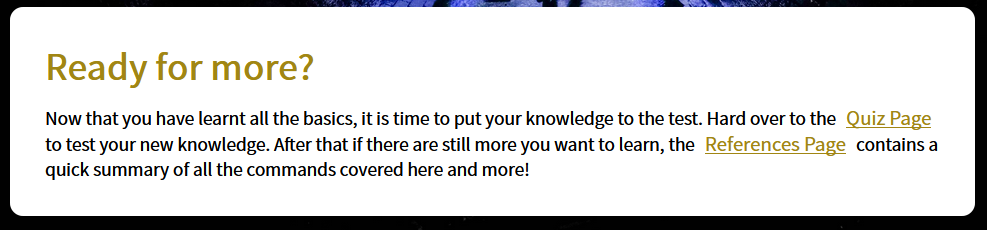
\includegraphics[width=0.8\linewidth]{web2}
	\caption{Screenshot of the link used in a content block}\label{fig:website}	
\end{figure}


\subsubsection{Attention}
Sometimes a possible feature is not always easily identifiable from a website and requires some way of identifying the user that there are more actions that can be done to better improve their viewing experience. This form of grabbing attention is completed through a bouncing the item very slightly. The bouncing should be smooth and not distracting from normal reading but upon scanning the entire page it should alert the user. Each individual bouncing element should also be interactive in some way, for example a docked menu can bounce and upon mousing over the menu will appear.

\subsubsection{Code Blocks}
% spaced and colored so easily caught to the eye when scrolling
Large chunks of code will be represented using the grey colour tones (as noted in Section~\ref{sec:color}). This toned and padded content will allow for code to be easily identified when skimmed through. The goal of code blocks is to be easily identified with the title of each content blocks. Figure~\ref{fig:codeblock} shows an screenshot of the code block in use on the main page.

\begin{figure}
	\centering
	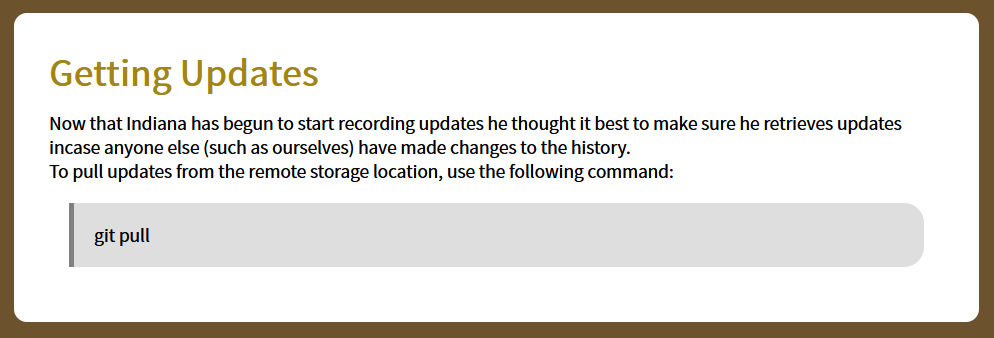
\includegraphics[width=0.8\linewidth]{web1}
	\caption{Screenshot of the code block used in a content block}\label{fig:codeblock}
\end{figure}


\subsubsection{Background}
% images and colors are washed out or dark so that the user is drawn to the content first and the background is just an after thought
The website should use by default a dark background color as defined in Section~\ref{sec:color}. The aim of this color choice is to ensure it both complements the primary color as well as placing focus on the content foremost.\\\\
An alternative background is allowed with a background image. If a background image is used than the image should be a basic image with minimal activity and can be washed out if required. This is so that the image follows the same goals as the plain background color, however in addition the background image should never be repeated or feature any transitions/features independent of the content. These additional features could draw attention away from the content and leave the user distracted, however simple and non-distracting animations could be used but not in excess as to distract the user away. Figure~\ref{fig:image} demonstrates the style of image to be used as well as how the content is still represented as the forefront and the background image is purely used for aesthetics.

\begin{figure}
	\centering
	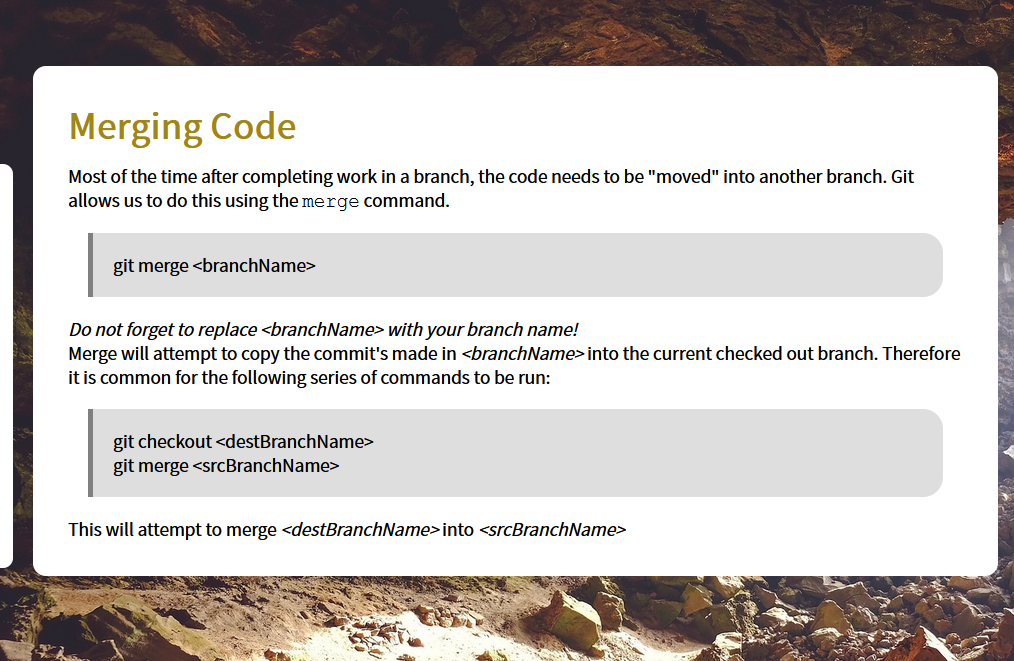
\includegraphics[width=0.8\linewidth]{background}
	\caption{Screenshot of the use of a background image behind content}\label{fig:image}
\end{figure}

\subsubsection{Smooth Hovering}
% all hover effects are meant to appear smooth and with no sudden movements. Site is for people just beginning and they dont want to be scared off. Animations not too slow that it is unusable for the experienced person 
A lot of the content being delivered is often perceived as difficult or challenging to learn by users, with a massive learning curve. So the aim of this site is to not go too fast and to not overwhelm people with quick movements. Therefore all actions should be animated or have a transition applied. These animations should occur for roughly 300 milliseconds, with an ease timing curve. These settings are aimed to help provide the smoothest transition possible while still appearing to be snappy. The ease timing curve helps to make the starting and end appear smooth while the middle filling bit quicker, therefore the user sees the larger defining changes more while still having an overall quick effect. Overall achieving the desired user transitions will help to provide a great \gls{ux}.

\subsection{Aesthetics User Testing}
% Reflect on the success of the Aesthetics User Testing design activity you did in Week 9
% Include screenshots of the mockups you used for the activity
% Include the testing plan you developed for the activity
% What feedback did you get and how did it inform your aesthetic decisions?
\subsubsection{Landing Page}
\begin{figure}[H]
	\centering
	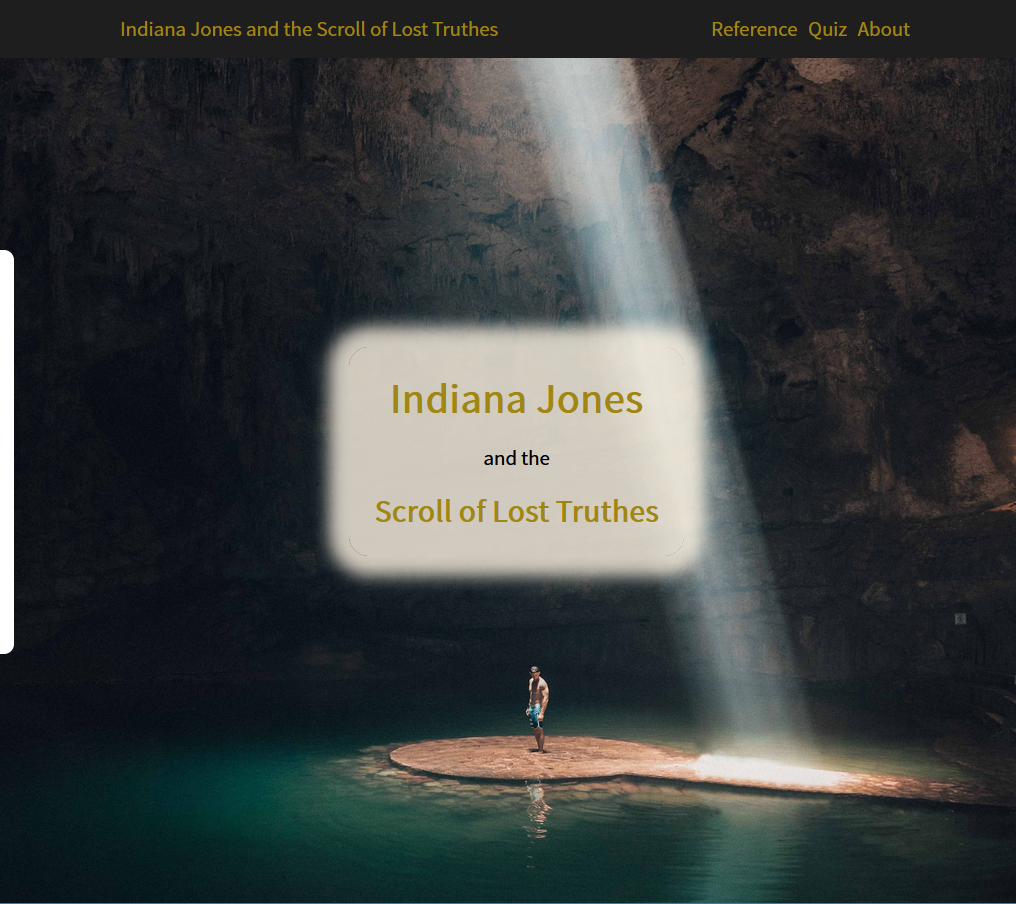
\includegraphics[width=0.8\linewidth]{homepage}
	\caption{Aesthetic example of the main landing page with content available on scroll}\label{fig:homepage}
\end{figure}
An important aspect of web-design is being able to capture and engage your audience from the very beginning. People browsing the internet are rarely forgiving for design and so it is important that people are engaged immediately. The aim of this test was to receive feedback from users about their thoughts on the site and if they are interested to know more.\\\\
Figure~\ref{fig:homepage} shows the initial mockups used to test people's responses. Almost everyone pointed out that due to the use of the colour and font sizing on the title, there were caught immediately. The second drawing factor is the lack of information partnered with the interesting title. Everyone wanted to know more and learn more about what was on the page. However all of the keen interest was suddenly directed to confusion when the question was raised about what to do next, the lack of direction and indication of actions on the site left people losing interest.

\subsubsection{Detailed Content Example}
\begin{figure}[H]
	\centering
	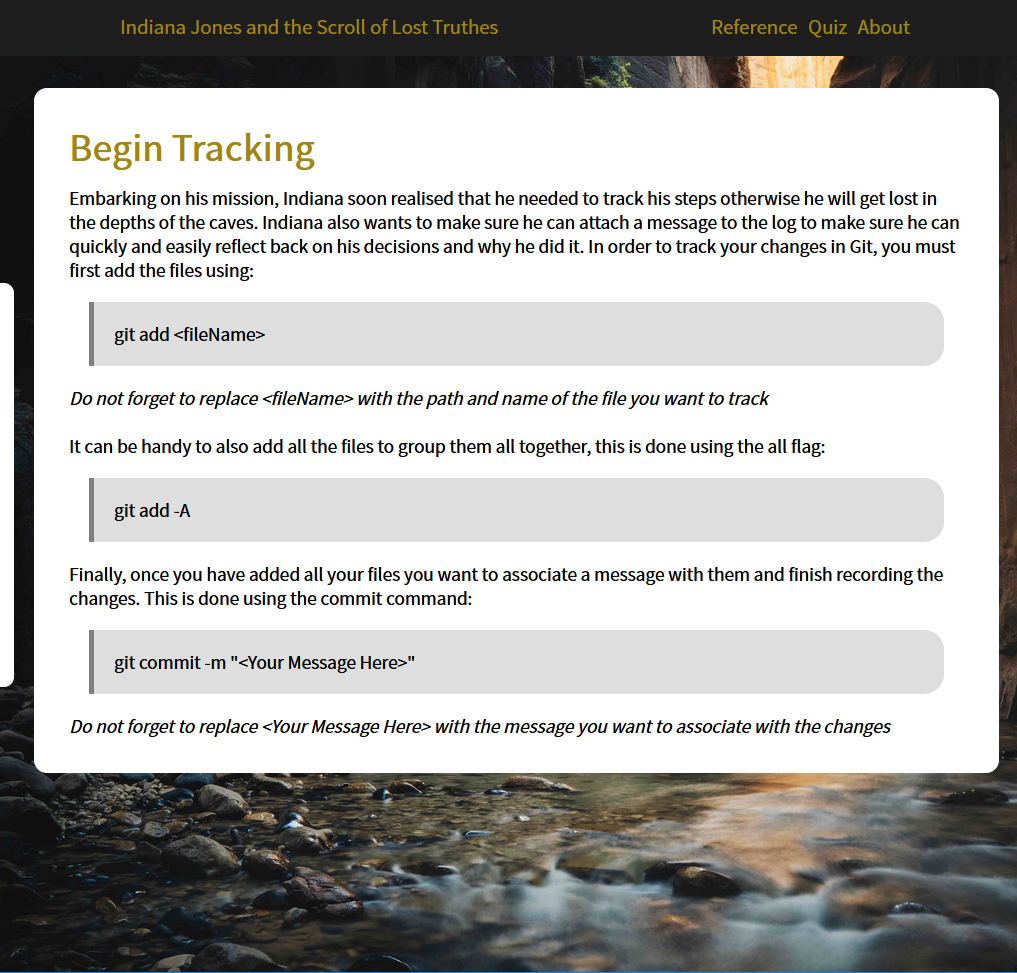
\includegraphics[width=0.8\linewidth]{examplepage}
	\caption{Aesthetic example of a page with a lot of detailed content}\label{fig:content}
\end{figure}
Another important test is the deliver of content and people's feedback on the choice of spacing and delivery of content. Figure~\ref{fig:content} is a screenshot of the mockup produced to users. All users liked the use of the white background on-top of the background image, with the black foreground text. Everyone found it easy to concentrate on the content and did not find it distracting. It was noted that the font sizing and spacing helped to break up the content into smaller sections which were easier to consume. Not everyone was aware of the use of the grey box and what they represented, however for people with some extensive computer knowledge they were able to see the metaphor between existing computer tutorials.

\subsubsection{References Page with Table Layout}
\begin{figure}[H]
	\centering
	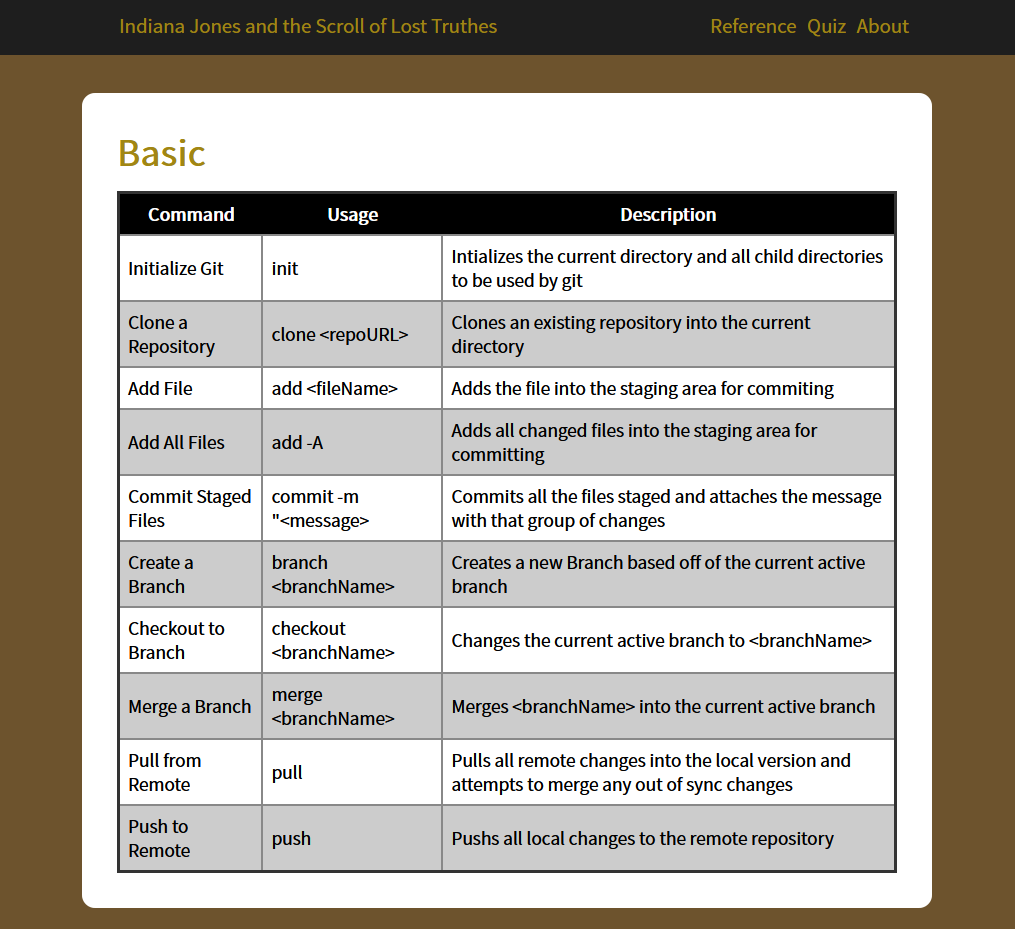
\includegraphics[width=0.8\linewidth]{refs}
	\caption{Aesthetic presentation of the references page, showing some basic commands}\label{fig:refs}
\end{figure}
Figure~\ref{fig:refs} was used to check the colour scheme and colour variability for a table being represented on the page. The aim of this test was to get user feedback around the styling of the table and if it fits within the style of the rest of the website. A lot of people agreed that the style of the table was simple and intuitive, however most people noted that the table as a whole does not fit the general style of the website. The website is more based around smooth and clean edges, while the table has hard and sharp corners.

\subsubsection{Quiz Git Sandbox}
\begin{figure}[H]
	\centering
	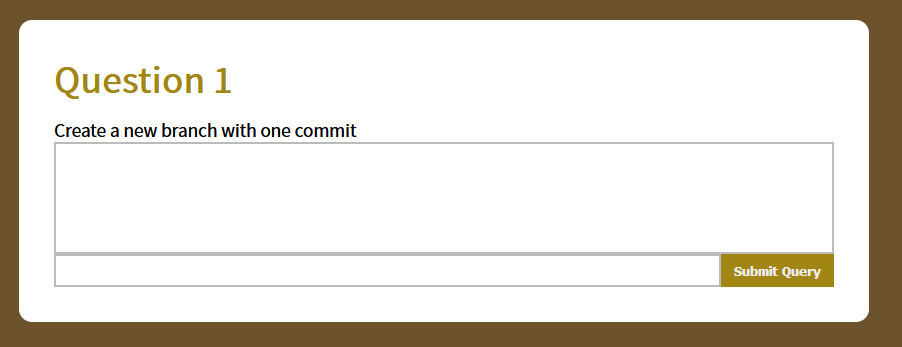
\includegraphics[width=0.8\linewidth]{terminal}
	\caption{Aesthetic layout of the \gls{git} sandbox}\label{fig:sandbox}
\end{figure}
The final aesthetics test was centred around getting feedback on the \gls{git} Sandbox control which is used in the Quiz page. This control is to allow people to test their basic \gls{git} knowledge in an environment which can do no harm to their system. Everyone that is unfamiliar with programming languages' tutorials did not understand the control and how to use it. The feedback provided was there was no clear place to begin and leave with the device. Some simple tooltips and differentiation between the top half and the bottom half.
